\chapter{质点动力学(二)}
有了力的定律和牛顿定律,运动学的根本任务,即在一定环境下求解物体的运动问题,似乎就成为求解运动方程$m\ddot{\vec{r}}=\vec{F}(\vec{r},\dot{\vec{r}},t)$的数学问题了。但如果我们在动力学定律的基础上引进一些新的概念,如动量、角动量、动能、势能、机械能等,就可以进而得到关于这些量的新的规律。而直接用这些规律去分析质点的运动问题,往往比从牛顿定律出发更为方便。这些新的规律就是所谓运动定律以及由此列出的守恒定律。有时即使力的具体形式不十分清楚(如约束力,碰撞中质点间的作用力等)这种方法也能为我们求解问题提供一定信息。再者牛顿定律只适用质点,不能直接用于质点组,特别是由大量质点组成的体系,若我们用牛顿定律去求解体系中每个质点的运动,计算将十分复杂,甚至无法进行,而利用关于动量、角动量、能量的规律,却可以使我们不必求解每个质点运动的情况下,获得关于质点组运动的许多知识。事实上运动定理及守恒定律几乎是我们解决质点组动力学问题的唯一可以利用的工具。

关于动量、角动量、能量的运动定理以及守恒定律虽然最初是经典力学中由牛顿定律演绎出来的,但物理学的发展表明,动量、角动量、能量这些概念,有关它们的定理以及守恒定律却可以推广到物理学的其他领域,如研究电磁现象、热现象、量子现象,因而这些定理以及守恒定律有着更普遍的意义。

动量、角动量、能量等等这些力学量都可以视作状态量,或状态函数。以后在分析力学中引入的拉格朗日函数、哈密顿函数都可作为状态函数,不过是特别的状态函数(特性函数)。

质点由一种状态按照运动规律变为另一种\underline{状态},在物理学中称为一个过程。系统运动状态变化是由于一个过程中,系统与外界的相互作用(以及系统内部的相互作用)导致的,因此描述质点运动状态的物理量的改变是由过程中外界的作用(以及系统内部相互作用)过程所决定的。因此描述质点运动状态的物理量的改变,应该是有过程中外界的作用(以及系统内部相互作用)过程所决定的。即应该有状态量的改变=过程量。这就是著名的牛顿-莱布尼茨公示。
\begin{align}
\text{牛顿-莱布尼茨公式:}u(t_2)-u(t_2)&=\int_{t_1}^{t_2}f(t)dt\notag\\
\text{状态量的改变}&=\text{过程量}\notag
\end{align}
经典力学中有许多规律都可以表达为这种形式,许多重要的物理量也是通过类似的表达式引入的。下面我们将从牛顿的运动方程$m\frac{d^2\vec{r}}{dt^2}=\vec{F}$出发,讨论可以演绎出哪些类似的关系,并相应的引入新的物理量。

\section{动量、动量定理、动量守恒定律}
\subsection{动量、动量定理}
若质点的质量$m$为常数,则:
\[m\frac{d\vec{v}}{dt}=\vec{F}\ \Rightarrow\ \frac{d(m\vec{v})}{dt}=\vec{F}\]
令$\vec{p}=m\vec{v}$,则下式即为动量定理:
\begin{align}
\frac{d\vec{p}}{dt}&=\vec{F}\notag\\
\vec{p_2}-\vec{p_1}&=\int_{t_1}^{t_2}\vec{F}(t)dt=\vec{I_{12}}\notag\\
\text{动量的改变}&=\text{外力的冲量}\notag
\end{align}

其中$I_{12}$记作在$[t_1,t_2]$时间内外力的冲量。

质点在做匀速运动时,其惯性质量不再是常数。$m=m(\vec{v})$,但此时动量定理仍然适用。这说明在这种条件下牛顿方程必须修改,这一点也证明动量概念,动量定理较牛顿运动方程有更普遍的意义。我们将在后面狭义相对论部分进一步讨论这个问题。
\subsection{动量守恒定律}
若$\vec{F}(t)=0$,则:
\[I_{12}=\int_{t_1}^{t_2}\vec{F}dt=0\ \Rightarrow\ \vec{p_2}-\vec{p_1}=0\]
\[\vec{p}(t)=\vec{p}(0)=\vec{p_0}\]

动量守恒的概念在讨论质点组,特别是由两个质点组成的系统的运动问题时特别有用。若质点组织存在内部相互作用,由于牛顿第三定律,两个质点的相互作用的作用力和反作用力大小相等方向相反,$F_{12}=-F_{21}$,质点组各质点所受的总的冲量等于零,因此质点组的总动量$\vec{P}$守恒:
\[\vec{P}=(\vec{P_1}+\vec{P_2}+\dots)=\vec{P_0}\]

\subsection{动量定理、动量守恒定律应用于质点组}
\subsubsection{内力和外力、主矢量}
\begin{description}
\item[内力]质点组内任意两个质点之间的作用力,例如第$j$个质点对第$i$个质点有作用力,记作$\vec{F}_{ij}^{in}$;注意到由牛顿第三定律,$\vec{F}_{ij}^{in}=-\vec{F}_{ji}^{in}$
\item[外力]质点组任一质点所受的外界作用力,例如第$i$个质点受外界作用力,记作$\vec{F}_i^{ex}$
\item[主矢量]记作$\vec{F}^{ex}$,定义为$\vec{F}^{ex}=\sum_i \vec{F}_i^{ex}$
\end{description}
\subsubsection{质点组的总动量、质点组动量定理、总动量守恒}
\begin{description}
\item[总动量]记作$\vec{p}$,定义为$\vec{p}=\sum_i \vec{p_i}$
\item[质点组的动量定理]
\begin{align}
\frac{d\vec{p}}{dt} &=\sum_i \frac{d\vec{p_i}}{dt} = \sum_i (\vec{F}_i^{ex} + \sum_{j\ne i}\vec{F}_{ij}^{in}) \notag \\
&=\sum_i \vec{F}_i^{ex}+\sum_{ \substack{i,j \\ i\ne j}}\vec{F}_{ij}^{in} = \vec{F}^{ex} \notag
\end{align}
\[\frac{d\vec{p}}{dt}=\vec{F}^{ex}\ \Rightarrow\ \vec{p_2}-\vec{p_1}=\int_{t_1}^{t_2}\vec{F}^{ex}dt\]
\end{description}
\subsubsection{总动量守恒定律}
\[\text{若}\vec{F}^\text{ex}=0,\ \text{则}\vec{p_2}-\vec{p_1}=0\text{,总动量守恒}\]
\subsection{质心、质心运动定理、质心参照系}
\subsubsection{质心}(质量中心)$(M,\vec{r_c})$

质心是这样一个质点,它集中了质点组的全部质量,它的动量等于质点组的总动量
\[M=\sum_i m_i\]
\[\vec{p}=\sum_i \vec{p_i}=\sum m_i \frac{d\vec{r_i}}{dt}=\frac{d}{dt}(\sum_i m_i\vec{r_i})=M\frac{d\vec{r_c}}{dt}=M\vec{v_c}\]
\[\vec{r_c}=\frac{\sum_i m_i\vec{r_i}}{M}\text{表示质心的位置},\  v_c=\frac{d\vec{r_c}}{dt}\text{表示质心的速度}\]
\subsubsection{质点参照系}(对某一个质点组而言)
把原点取在质点上,坐标轴的方向始终与某一惯性系坐标轴保持平行的平动参照系叫做质点参照系,有时也称质点坐标系,或简称质心系。判断质心系是否是惯性系,只需判断质点系中的速度相对惯性系中是否为匀速。记$\vec{r_i'}$为相对质心系的位置矢量。

对于不受外力作用的体系(孤立系)或受外力的矢量和(主矢)为零的体系,其质心系为惯性系;否则,则为非惯性系。在讨论质点组动力学问题时,质心系具有一系列特点。在质心系中,质点组的总动量恒为零。
\begin{align}
\vec{r_i'}&=\vec{r_i}-\vec{r_c} \notag \\
\vec{v_i'}&=\vec{v_i}-\vec{v_c} \notag \\
\vec{p'}&=\sum_i m_i \vec{v_i'}=\sum_i m_i(\vec{v_i}-\vec{v_c}) = \vec{p}-M\vec{v_c}=0 \tag{*}
\end{align}
由(*)式可见,从质心系看,质点组的总动量恒为0
\subsubsection{质心系处理两体问题}
\subsection{例题分析}
\subsubsection{人船模型}
质量为$M=500kg$,长为$4m$的木船漂浮在静止的水面上,船尾站着一个质量为$50kg$的人,若人从船尾走到船头,问船相对于水面走了多少?
\begin{figure} [ht]
\centering
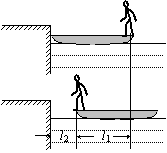
\includegraphics[scale=.6]{renchuan.png}
\caption{\simsun 人船模型}
\label{renchuan}
\end{figure}

\begin{enumerate}
\item 若船与水的摩擦力可以忽略,则此时人与船的总动量守恒
\[m\vec{v}+M\vec{v'}=0\]
\[\Rightarrow\int_{t_s}^{t_f}mvdt-\int_{t_s}^{t_f}Mv'dt=ml_1-Ml_2=0\]
因为是从船尾走到船头,所以人相对于船的位移为船长
\[L=l_1+l_2\]
因此
\[m(L-l_2)-Ml_2=0\]
\[\Rightarrow l_2=\frac{mL}{m+M}=\frac{4}{11}m\]
注意到船移动过程中,质心位移不变。
\item 若船与水的摩擦力不能忽略,并设阻力与船相对水的速度成正比,即$f=-\alpha\vec{v}$,并假设人以相对于船的恒定速率$v'$从船尾走到船头,分析船的运动可分为4个阶段:\begin{description}
\item[第一阶段]在极短的时间内,人从静止达到速度$v'$(相对船),同时船也从静止达到速度$V_{10}$,此阶段可忽略阻力(阻力的冲量趋近0),可用动量守恒。
\[m(v'+v_{10})+Mv_{10}=0\]
\item[第二阶段]人以速度$v'$(相对船)从船尾走到船头,此阶段必须考虑水的阻力的作用。
\[m\frac{d}{dt}(v'+v)+M\frac{dv}{dt}=-\alpha v\]
从$t=0$到$t=\frac{2}{v'}$求积分得到$v_{1f}$
\item[第三阶段]在极短的时间内,人在船尾定住,仿前,此阶段仍可忽略阻力,用动量守恒定律。
求$v_{20}$
\[m(v'+v_{1f})+Mv_{1f}=(m+M)v_{20}\]
\item[第四阶段]由于阻力的租用人和船一起由速度$V{20}$趋向速度$V_{2f}=0$
\[(m+M)\frac{dv}{dt}=-\alpha v\]
\end{description}
\end{enumerate}
\subsection{变质量物体的运动方程}
\subsubsection{体系的选择,主体,附体}
变质量物体运动过程分解为一系列元过程,在分析元过程时,在$\varDelta t$时间内由主体(设被考察变质量物体的质量为m),由于吸入(或抛开)附体(设其质量为$\varDelta m$)而合二为一(或一分为二)。
\subsubsection{变质量物体的运动过程}
\begin{align}
(m+\varDelta m)(\vec{v}+\vec{\varDelta v})-(\varDelta m\vec{u}+m\vec{v}) &= \vec{F}\varDelta t \notag \\
m\vec{v}+\varDelta m\vec{v}+m\vec{\varDelta v}+\varDelta m\vec{\varDelta v}-\varDelta m\vec{u}-m\vec{v}&= \vec{F}\varDelta t \notag \\
\end{align}
化简,舍去$\varDelta m\vec{\varDelta v}$这个二阶小量得
\begin{align}
m\vec{\varDelta v}+\varDelta m(\vec{v}-\vec{u})&=\vec{F}\varDelta t \notag \\
m\frac{d\vec{v}}{dt}+\frac{dm}{dt}(\vec{v}-\vec{u})&=\vec{F} \notag
\end{align}
\[\begin{cases}
\frac{dm}{dt}>0\quad\text{如:雨滴}\\
\frac{dm}{dt}<0\quad\text{如:火箭}\\
\end{cases}\]

\subsubsection{火箭的运动}
令$\vec{u}-\vec{v}=\vec{v_r}$,则$\vec{v_r}$表示燃料相对火箭的速度,若忽略$\vec{F}$的作用,运动方程为:
\begin{align}
m\frac{d\vec{v}}{dt}&=\vec{v_r}\frac{dm}{dt} \notag\\
mdv&=-v_rdm \notag\\
dv&=-v_r\frac{dm}{m} \notag\\
\int_{v_0}^{v_f}dv&=-v_r\int_{M_0}^{M_f}\frac{dm}{m} \notag\\
v_f-v_0&=-v_r(\ln M_f-\ln M_0)\notag\\
&=v_r\ln \frac{M_0}{M_f}=v_r \ln N\notag
\end{align}
最终结论为:
\[v_f-v_0=v_r\ln N\]
其中$N$为初末时刻的质量比,$N=\frac{M_0}{M_f}$;特别地,当$v_0=0$:
\[v_f=v_r\ln N\]
\[v_r \thickapprox
\begin{cases}
2km/s\text{,常规燃料}\\
4km/s\text{,非常规燃料}\\
\end{cases}\]
例如阿波罗三级火箭:
\begin{description}
\item[第一级] $v_{r_1}\thickapprox 2.9km/s,N_1=16$
\item[第二三级] $v_{r_2} \thickapprox 4km/s,N_2=14,N_3=12$
\[v_f=v{r_1}\ln N_1+v_{r_2}(\ln N_2+\ln N_3) = 28.5km/s\]

较著名的运载火箭
\begin{enumerate}
\item 中国:长征三号、长征四号
\item 美国:土星五号、大力神号
\item 欧洲:亚娜5型
\end{enumerate}

目前欧美的火箭已经能将有效载荷6吨以上送入地球同步轨道。
\end{description}
\section{动能与势能}
研究动力学问题,就要研究相互作用,既要看到里可以改变质点的动量(力的时间积累效应——冲量),也要看到里可以改变质点的动能(力的空间积累效应——功)。

对于质点组的动力学问题,既要研究质点组与外界的相互作用,也要研究质点组内部的相互作用。

质点组内部的相互作用,在许多情况下,如万有引力、弹性力、库仑力等都可以表示为两质点见相对位置的函数,这时体系内部相互作用力所做的功可以表述为体系的势能的改变。

这样对于质点组,除了上一节所介绍的动量概念外,还可以用动能,相互作用势能,机械能等等概念基于系统更细微,更完善的描述。而这些物理量的变化规律用动能定理,动能关系等等来表述。

质点组与外界相互作用时,既包含了动量的转移与交换(上一节内容),也包含了解量的转移与交换(本节内容),还包括了角动量的转移与交换(下一节内容),这样从不同层面反映了系统与外界相互作用时所包含的物理内容。

\[\text{动力学问题要研究的相互作用}
\begin{cases}
\text{力的时间积累效应(冲量)引起了动量的变化}\\
\text{力的空间积累效应引起了体系能量的变化}
\end{cases}\]
\subsection{动能、动能定理}
\subsubsection{质点的动能、动能定理}
\begin{align}
m\frac{d\vec{v}}{dt}=\vec{F} \ &\Rightarrow \ m\frac{d\vec{v}}{dt}\cdot\vec{v}=\vec{F}\cdot\vec{v} \notag\\
&\Rightarrow m(\frac{dv_x}{dt},\frac{dv_y}{dt},\frac{dv_z}{dt})\cdot(v_x,v_y,v_z)=\vec{F}\cdot\vec{v} \notag\\
&\Rightarrow \frac{d}{dt}(\frac{1}{2}m(v_x^2+v_y^2+v_z^2))=\vec{F}\cdot\vec{v} \notag\\
&\Rightarrow \frac{d}{dt}(\frac{1}{2}mv^2)=\vec{F}\cdot\vec{v} \notag\\
&\Rightarrow \frac{d}{dt}(E_k)=P \notag
\end{align}
\begin{align}
\varDelta E_k&=\underset{(c)}{\int_{\vec{r_1}}^{\vec{r_2}}}\vec{F}d\vec{r} \notag \\
\text{状态量的改变}&=\text{过程量}\notag
\end{align}
\subsubsection{功的计算}
定义元功:$dA=\vec{F}\cdot d\vec{r}$
\begin{align}
d\vec{r}&=dx\vec{i}+dy\vec{i}+dz\vec{k}\quad\text{(直角坐标系下)}\notag\\
dA&=F_xdx+F_ydy+f_zdz\notag\\
d\vec{r}&=dr\vec{e_r}+rd\theta\vec{e_\theta}+r\sin\theta d\varphi\vec{e\varphi}\quad\text{(球坐标系下)}\notag \\
dA&=F_rdr+F_\theta d\theta+F_\varphi r\sin\theta d\theta \notag
\end{align}
\begin{description}
\item[重力的功]
\[F_x=0 \quad F_y=0 \quad F_z=-mg \]
\begin{align}
F&=-mg\vec{k} \notag \\
dA&=-mgdz\notag\\
\int_a^b dA&=-mg\int_{z_a}^{z_b} dz\notag\\
&=-mg(z_b-z_a)\notag\\
&=mg(z_a-z_b)\notag
\end{align}
\item[万有引力的功]
\begin{align}
\vec{F}&=-\frac{GMm}{r^2}\vec{e_r}\notag\\
dA&=-\frac{GMm}{r^2}dr\notag\\
\int_a^b dA&=-\int_{r_a}^{r_b} \frac{GMm}{r^2} dr\notag\\
&= -GMm(-\frac{1}{r})|_{r_a}^{r_b}\notag\\
&=\frac{GMm}{r_b}-\frac{GMm}{r_a}\notag
\end{align}
\item[弹力的功的计算(一维情形)]
\begin{align}
\vec{F}&=-k\vec{x}=-kx\vec{i}\notag\\
dA&=-kxdx\notag\\
\int_a^b dA&=\int_{x_0}^{x_f}(-kx)dx\notag\\
&=-k(\frac{1}{2}x^2)|_{x_0}^{x_f}\notag\\
&=\frac{1}{2}kx_0^2-\frac{1}{2}kx_f^2\notag
\end{align}
\end{description}
\subsubsection{质点组动能、质点组动能定理}
\begin{description}
\item[质点组动能]\[E_k=\sum_i \frac{1}{2}m_iv_i^2\]
\item[质点组的动能定理]\[\frac{dE_k}{dt}=\sum_i \vec{F_i}\vec{v_i}\]
\begin{align}
E_{k_f}-E_{k_0}&=\sum_i A_i\notag\\
&= \sum_i \underset{(c)}{\int_{\vec{r_0}}^{\vec{r_f}}} \vec{F_i}d\vec{r_i} + \sum_{\substack{i,j\\i\ne j}}\vec{F}_{ij}^{in}\notag \\
&=A^{ex}+A^{in} \notag
\end{align}
\[A^{ex}=\sum_i \underset{(c)}{\int_{\vec{r_{i0}}}^{\vec{r_{if}}}}\vec{F}_i^{ex}d\vec{r_i}\]
\[A^{in}=\sum_i A_i^{in} = \sum_i\underset{(c)}{\int_{\vec{r_{i0}}}^{\vec{r_{if}}}}\sum_{\substack{i,j\\i\ne j}} \vec{F}_{ij}^{in} d\vec{r_i}\]
考虑第$i,j$个质点相互作用力所做的功:
\begin{align}
\vec{F}_{ij}^{in}d\vec{r_i}+\vec{F}_{ji}^{in}d\vec{r_j} &= \vec{F}_{ij}^{in}(d\vec{r_i}-d\vec{r_j}) \notag\\
&=\vec{F}_{ij}d\vec{r_{ji}}\notag
\end{align}\begin{align}
d\vec{r_i}+(\vec{r_{ij}}+d\vec{r_{ij}})+(-d\vec{r_j})+(-\vec{r_ij})&=0 \notag\\
d\vec{r_i}-d\vec{r_j}&=-d\vec{r_{ij}}\notag
\end{align}
\[\therefore A^{in}=\sum_{i<j}\underset{(c)}{\int_{\vec{r_{i0}}}^{\vec{r_{if}}}}\vec{F_{ij}}d\vec{r_{ji}} \]
\end{description}

作用力与反作用力这一对内力的总功只与两质点相对距离的变化$dr_{ij}$有关,在牛顿时空中,两质点相对距离的变化与参照系无关。因此内力的总共与参照系无关。

前面的例子,与其中一个质点相对静止的参照系中,作用于另一个质点的力仅与该质点的始末位置有关,而对该质点所经的具体路径无关。当然如果内力为耗散力就与路径有关了。
\subsection{质点组的势能}
\subsubsection{保守力和非保守力}
定义:作用在质点上的力$\vec{F}$,当质点由空间任一位置经过闭合路径$c$回到出发位置,$\vec{F}$所做的功恒为$0$,亦即
\[\oint\vec{F} d\vec{r}=0\]
则称$\vec{F}$为保守力,否则称非保守力。
\[\begin{cases}
\text{保守力如:万有引力,弹性力,库伦静电力}\\
\text{非保守力如:摩擦力($\oint \vec{F_\mu}d\vec{r}<0$),电路内的非静电力($\oint \vec{F}_\text{非静电力}d\vec{r}>0$)}
\end{cases}\]

保守体系:
若质点组内任一两质点间的作用力都是保守力,则称该质点组为保守体系。
\subsubsection{质点组的势能(两质点保守体系)}
设初始时两只点位置分别为$\vec{r_{10}},\vec{r_{20}}$,记为$\mathbf{a}=(\vec{r_{10}},\vec{r_{20}})$,经过一段时间,两质点分别到达位置$\vec{r_{1f}},\vec{r_{2f}}$,记为$\mathbf{b}=(\vec{r_{1f}},\vec{r_{2f}})$。由于两质点间的相互作用力,对两质点作的总功与路径无关,只与始末点位置有关,记为:\[A_{a\to b}\text{(保守力)} = -(E_p(\mathbf {a})-E_p(\mathbf {b}))\]
我们把$E_p(a),E_p(b)$称为质点组于位置$\mathbf{a}$和位置$\mathbf{b}$处的势能。由上式可知,$E_p(\mathbf{a}),E_p(\mathbf {b})$可差任一常数。保守力作用下两质点体系与这种与相对位置联系的做功本领称作保守体系的势能(或位能)。
\subsubsection{势能图,势能曲线}
\begin{description}
\item[势能图]表示势能与两质点相对位置关系的图形叫势能图
\item[势能曲线]若势能仅与相对位置的一个坐标有关,势能与该坐标的关系图形表示即为势能曲线
\begin{description}
\item[重力势能曲线]$\ $
\begin{figure} [ht]
\centering
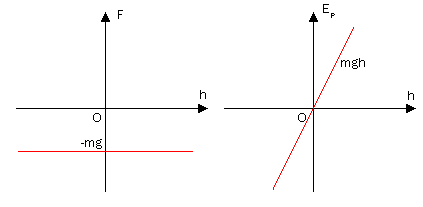
\includegraphics[scale=.6]{PotentialEnergy_Gravitational2.png}
\caption{\simsun 重力势能曲线}
\label{PotentialEnergy_Gravitational2}
\end{figure}
\item[弹力势能曲线]$\ $
\begin{figure} [ht]
\centering
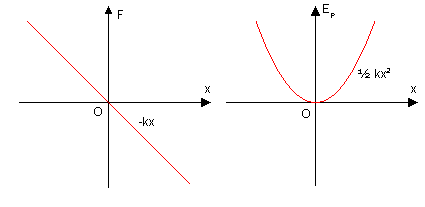
\includegraphics[scale=.6]{PotentialEnergy_Elastic.png}
\caption{\simsun 弹力势能曲线}
\label{PotentialEnergy_Elastic}
\end{figure}
\item[引力势能曲线] $\ $
\begin{figure} [ht]
\centering
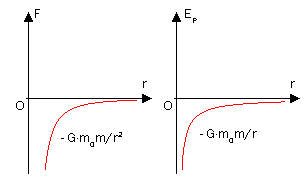
\includegraphics[scale=.6]{PotentialEnergy_Gravitational1.png}
\caption{\simsun 引力势能曲线}
\label{PotentialEnergy_Gravitational1}
\end{figure}
\item[双原子分子势能曲线]
\newpage
\begin{figure} [ht]
\centering
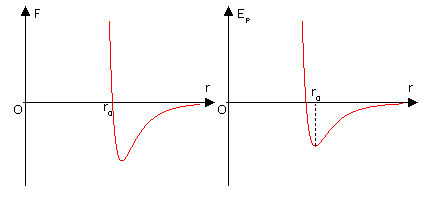
\includegraphics[scale=.6]{PotentialEnergy_Intermolecular.png}
\caption{\simsun 双原子分子势能曲线}
\label{PotentialEnergy_Intermolecular}
\end{figure}
\end{description}
\end{description}
\subsection{功能关系,机械能及其守恒定律}
\subsubsection{质点组的机械能,功能关系}
$A^{ex}$表示外力做功,则质点组的动能定理表述为:
\[E_{k_f}-E{k_0}=A^{ex}+A^{in}\]
\[A^\text{in}=A^\text{in}_\text{保守}+A^\text{in}_\text{非保守}\]
\[A^\text{in}_\text{保守} = -(E_{p_f}-E_{p_0})\]
\begin{align}
\therefore E_{k_f}-E_{k_0}&=-(E_{p_f}-E_{p_0})+A^\text{in}_\text{保守}+A^{ex} \notag \\
(E_{k_f}+E_{k_p})-(E_{k_0}+E_{p_0}) &= A^\text{in}_\text{保守}+A^{ex} \notag \\
E_f-E_0&= A^\text{in}_\text{保守}+A^{ex} \notag \\
\text{质点组的机械能之差}&=\text{外力的功}+\text{非保守内力的功}\notag
\end{align}
\subsubsection{机械能守恒}
若外力不做功($A^{ex}=0$)且非保守内力不做功($A^{in}_\text{非保守}=0$,没有动能转化为内能)则有
\[E_f-E_0=0\]
即
\[E_f=E_0=\text{恒量}\]
\subsubsection{$M\gg m$的两质点的孤立保守系的机械能守恒}
特点:
\begin{enumerate}
\item 机械能守恒:\[\frac{1}{2}MV^2+\frac{1}{2}mv^2+E_p(\vec{r}-\vec{R})=\text{恒量}\]
\item 质心系是惯性系:在质心系下
\[\begin{cases}
\vec{V}\ll\vec{v}:\quad M\vec{V}=-m\vec{v} \\
\vec{R}\ll \vec{r}:\quad M\vec{R}=-m\vec{r}
\end{cases}\]
\end{enumerate}
若$\frac{\frac{1}{2}MV^2}{\frac{1}{2}mv^2}=\frac{m}{M}(m\ll M)$,可以认为质心位置与$M$的位置相同,质点组的动能$=$小质点的动能。

设$E_p(\vec{r}_\text{相对})$表示在$M$产生的保守力场中的势能,此时:
\[\frac{1}{2}mv^2+E_p(\vec{r}_\text{相对})=\text{恒量}\]

即在质心系中,体系的动能表现为小质点的动能。体系的势能表现为仅由小质量质点的位置决定,即质量悬殊的两质点体系的机械能守恒表现为小指两质点的动能和势能之和为恒量。作为体系的另一部分,大质量质点在守恒定律表达式中似乎不出现。正是在这种意义下,我们会说到质点在保守力场中的机械能如机械能守恒定律。

在大质点物体($M$)的周围的空间,存在一种性质(物质),他表现为对外在着空间的任意位置的其他质点(其质量$m\ll M$)有力的作用,作用力的大小和方向完全有质量所在位置及其质量所决定,而且此力对质点所做的功仅有质点的始末位置决定,而与质点运动的具体路径无关。我们称这中间存在一种特殊的立场——保守立场,$M$是这力场的场源,而$M$对$m$的作用力则可称为保守立场对$m$的作用力。

地球对其表面附近物体的重力作用(重力场),地球对人造卫星的引力作用(引力场)都是保守力场,在原子物理中,氢原子中原子和对外围中子的静电力作用($M_p\gg m_e$)也属于保守立场。

对这样的体系的运动分析可归纳为单个质点在保守力场中的运动。

以及涉及质量在保守立场中的机械能以及机械能守恒定律

\[E=\frac{1}{2}mv^2+E_p=\text{恒量}\]

\subsubsection{质点在保守力场中机械能及其守恒定律}
\[\frac{1}{2}MV^2+\frac{1}{2}mv^2=\frac{1}{2}\mu(\vec{v}-\vec{V})^2\]
其中$\mu=\frac{Mm}{M+m}$称为约化质量。因为$\vec{v}\gg \vec{V}$,
\[\frac{1}{2}\mu (\vec{v}-\vec{V})^2+E_p(\vec{r}_\text{相对})=\frac{1}{2}\mu v^2+E_p(\vec{r}_\text{相对})=\text{恒量}\]

\subsection{质心系中的动能关系和机械能守恒定律}
\subsubsection{质心动能,柯尼希定理({\A Konig's theorem})}
设质点组各质点在某一参照系$S$的坐标为$\{\vec{r_i}\}$,在质心系$(c)$中的坐标用$\{\vec{r_i}'\}$表示,
\[\vec{r_i}=\vec{r_c}+\vec{r_i}' \quad \vec{v_i}=\vec{v_c}+\vec{v_i}'\]
\[E_k=\sum_i \frac{1}{2}m_i v_i^2 \quad E_{ck}=\frac{1}{2}MV_c^2\text{(质心在$S$系中的动能,$M=\sum_i m_i,\vec{r_c}=\frac{\sum_i m_i \vec{r_i}}{M}$)}\]
\[E_k=\sum_i \frac{1}{2}m_i v_i'^2\text{(质点组在质心系的动能)}\]
\[\text{三者关系:}E_k=E_{ck}+E_{kc}\]
\begin{theorem}[\simhei 柯尼希定理]
\simsun 质点系的总动能等于全部质量集中在质心时质心的动能,加上各质点相对于质心平动坐标系运动所具有的动能。
\end{theorem}
\begin{proof}[\simhei 证明]
\begin{align}
E_k=\sum_i \frac{1}{2}m_iv_i^2 &= \sum_i \frac{1}{2}m_i(\vec{v_c}+\vec{v_i}')(\vec{v_c}+\vec{v_i})\notag\\
&=\sum_i \frac{1}{2}m_i v_c^2+\sum_i \frac{1}{2}m_iv_i'^2+\sum_i \frac{1}{2}m_i 2\vec{v_c}\cdot\vec{v_i}'\notag
\end{align}
\begin{align}
\because&\ \sum_i \frac{1}{2}m_i2\vec{v_c}\cdot\vec{v_i}'=\vec{v_c}\cdot(\sum_i m_i\vec{v_i}')\text{\simsun ,在质心系中动量和为$0$}\notag\\
\therefore&\ \sum_i m_i\vec{v_i}'=0\notag\\
\therefore&\ \sum_i \frac{1}{2}m_i2\vec{v_c}\cdot\vec{v_i}'=0 \notag\\
\therefore&\ E_k=E_{ck}+E{kc}\notag
\end{align}
\end{proof}
\subsubsection{质心系中的动能关系和机械能守恒定律}
惯性参考系中:
\[E_f-E_0=A^{ex}+A^{in}_{\text{非保守}}\]
若质心系是惯性系:
\[E_f’-E_0‘=A^{ex}’+A^{in}_{\text{非保守}}‘\]
且若质心系是非惯性系时也成立,因为$A'_\text{惯性力}=0$,设质心对某惯性系的加速度$\vec{a}$,每一个质点在质心系中所受的惯性力为$-m_i\vec{a}$,惯性力所做的功
\[A'_\text{惯性力}=\sum_i(-m_i\vec{a})d\vec{r_i}=-\vec{a}\cdot(\sum_i m_i d\vec{r_i})=0\]
%\subsubsection{例题分析}
\subsection{碰撞}
\subsubsection{碰撞类型}
\[\begin{cases}\text{正碰,斜碰}\\
\text{弹性,非弹性碰撞}\begin{cases}\text{弹性碰撞:能量守恒}\\\text{非弹性碰撞:机械能损失}\begin{cases}
\text{一般非弹性碰撞}\\
\text{完全非弹性碰撞}
\end{cases}
\end{cases}
\end{cases}\]
\subsection{例题分析}

\section{角动量、角动量定理、角动量守恒定律}
这一节介绍另一个描述质点运动状态的物理量——角动量(又称动量矩)。当质点或体系作转动时,角动量是很重要的物理量。观察我们周围的世界,大到地球、太阳系、银河系、星系团,小到分子、原子,甚至是组成原子、分子的原子核、电子以及各层次的基本粒子,他们都在不停的“转动”着,而描述转动的最恰当的物理量是角动量。当体系有一个转动状态变为另一个转动状态,角动量要发生改变,这种改变由力矩、冲量矩决定,他们之间的联系由角动量定理来描述。

在物理世界中,常常遇到相互作用力是有心力的情况,有心力对力心的力矩、冲量矩等于零,因此在这种情况下,质点或系统关于力的角动量是守恒的,在宏观物理、微观物理中常常遇到这样的情况。
\begin{center}角动量是一个描述转动的物理量\end{center}
\subsection{角动量,角动量定理}
\[\frac{d\vec{p}}{dt}=\vec{F} \  \Rightarrow \ \vec{r}\times\frac{d\vec{p}}{dt}=\vec{r}\times\vec{F}\]
\[\text{注意到:}\frac{d}{dt}(\vec{r}\times\vec{p})=\frac{d\vec{r}}{dt}\times\vec{p}+\vec{r}\times\frac{d\vec{p}}{dt}=0+\vec{r}\times\frac{d\vec{p}}{dt}\]
\[\therefore \frac{d}{dt}(\vec{r}\times\vec{p}) = \vec{r}\times\vec{F}\]
定义$\vec{L}=\vec{r}\times\vec{p}$,称为质点相对于参考点$O$的角动量;定义$\vec{M}=\vec{r}\times\vec{F}$,称为质点所受外力相对于参考点$O$的力矩
\[\vec{L}=\vec{r}\times\vec{p}=m\vec{r}\times\frac{d\vec{r}}{dt}=2m\frac{d\sigma}{dt}\]
其中$\sigma$表示单位时间扫过的面积,$\vec{r}\times d\vec{r}=2d\sigma$,$\frac{d\sigma}{dt}$叫做面积速度;定义
\[\vec{L}=2m\vec{A}\]
$\vec{A}$称作面积速度
\[\vec{A}=\frac{d\sigma}{dt}\]
\subsection{质点组的角动量,质点组的角动量定理}
质点组的角动量定义为\[\vec{L}=\sum_i \vec{L_i}\]
\[\frac{d\vec{L}}{dt}=\sum_i \frac{dL_i}{dt}=\sum_i \vec{M_i} = \sum_i(\vec{M}_i^{ex}+\sum_{i\ne j} \vec{M}_{ij}^{in}) = \sum_i\vec{M}_i^{ex}\]
注意到$\sum_i \sum_{j\ne i} \vec{M_{ij}}^{in} = 0$
\[\vec{r_i}\times\vec{F_{ij}}+\vec{r_j}\times\vec{F_{ji}}=(\vec{r_i}-\vec{r_j})\times\vec{F_{ij}}=0\]
\[\Rightarrow \frac{d\vec{L}}{dt}=\sum_i \vec{M}_i^{ex}\]
\subsection{实验室系和质心系角动量之间的关系}
$\vec{L}=\vec{L_c}+\vec{L'}$
\[\vec{L}=\sum_i \vec{L_i},\vec{L_c}=\vec{r_c}\times\vec{p}=\vec{r_c}\times M\vec{v_0} = \sum_i \vec{r_i}\times\vec{p_i}\]
\[\vec{L'}=\sum_i \vec{L_i'}=\sum_i \vec{r_i'}\times\vec{p_i'}\]
\[\vec{r_i}=\vec{r_c}+\vec{r_i'},\vec{v_i}=\vec{v_c}+\vec{v_i'}\]
\begin{align}
\vec{L}&=\sum_i \vec{r_i}\times m\vec{v_i}=\sum_i (\vec{r_c}+\vec{r_i'})\times m(\vec{v_c}+\vec{v_i'})\notag \\
&=\vec{r_c}\times(\sum_i M_i\vec{r_i})+\sum_i \vec{r_c'}\times m \vec{v_i'}+\sum_i \vec{r_c}\times m_i \vec{v_i'}+\sum_i m_i \vec{r_i'}\times\vec{v_0} \notag \\
&=\vec{r_c}\times(\sum_i M_i\vec{r_i})+\sum_i \vec{r_c'}\times m \vec{v_i'}\notag
\end{align}
在质心系中$\sum_i m_i \vec{r_i'}=0,\sum_i m_i\vec{v_i'}=0$,推出
\[\vec{L}=\vec{L_c}+\vec{L'}\]
不论质心系是否是惯性系,在质心系中质点组的角动量定理仍然为
\[\frac{d\vec{L}'}{dt}=\sum_i \vec{M_i}^{ex}\quad(\sum_i \vec{M}_{i,\text{惯性}}=0)\]
\subsection{质点在有心力场中的运动}
\subsubsection{有心力、有心力场}
所谓有心力,就是方向始终指向(或被向)固定中心的力
\[\vec{F}=f(\vec{r})\vec{e_r}\]
$\vec{e_r}$为以固定中心为原点的矢径的单位矢量,而该固定中心成为力心。在大多数情况下,有心力的大小仅与考察点至力心的距离有关,即
\[\vec{F}=f(r)\vec{e_r}\]
这样的有心力称为中心对称有心力,这样的有心力是保守力,我们通常说的有心力指的就是这种中心对称的有心力。

前面去讨论$M\gg m$的二质点组成的保守体系时曾指出质心系与$M$静止参照系几乎等价。质心近似在$M$所在任意相互作用力,体系势能仅由$m$在$M$相对静止参照系中的位矢$\vec{r}$决定,可以推出:

在大质量周围的空间,存在一种性质(物质),他表现为对处于着空间的任意位置的其他质量(其质量$m\ll M$)有力的作用,作用力的大小和方向完全由质点所在位置及其性质(质量的,荷电量$q$等)所决定,我们称这空间存在一特殊的力场,$M$就是这力场的场源。若$M$对$m$的作用力是有心力,则称在$M$周围的空间存在有心力场。例如地球对其表面附近物体的重力作用,地球对人造卫星的引力作用,在原子中氢原子中原子核对外围电子的静电力作用,我们都可以表示为相应的对象在重力场、引力场、静电力场中所受的作用。而后两种情况都源于有心力场情形。
\subsubsection{有心力场中质点运动的一般特征——两个守恒量}
\begin{enumerate}
\item 角动量守恒:由于有心力对力心的力矩恒等于零
\[\vec{M}=\vec{r}\times f(r)\vec{e_r}=0\]
由质点角动量定理可知
\[\frac{d\vec{L}}{dt}=\vec{M}=0\quad \vec{L}=\vec{L_0}=\text{常量}\]
质点对于质心的角动量$\vec{L}$守恒
\[\vec{L}=\vec{r}\times\vec{p}=m\vec{r}\times\vec{v}=常矢量\]
$\vec{L}$的方向不变,质点必在由$\vec{r}\times\vec{v}$决定的平面内运动。

由此,讨论质点在有心力场中的运动,采用平面极坐标比较方便。$\vec{L}$的大小不变,$L=$常量。

在平面极坐标下,$\vec{v}=(\dot{r}\vec{e_r}+r\dot{\phi}\vec{e_{\phi}})$,$\vec{r}=r\vec{e_r}$
\[\vec{L}=\vec{r}\times\vec{p}=mr^2\dot{\phi} \vec{e_r}\times\vec{e_\phi}=mr^2\dot{\phi}\vec{k}\]
\[\vec{k}=\vec{e_r}\times\vec{e_\phi}\,\text{为垂直于质点轨道平面方向上单位矢量}\]
故有
\[L=mr^2\dot{\phi}=\text{常量}\]

\item 机械能守恒
由于有心力场是保守力场,可以引入势能函数$E_p$,由前,通常选择$r\to\infty$时为$E_p$的势能零点,则有
\[E_p^{(r)}=-\int_\infty^r f(r) dr = \int_r^\infty f(r) dr\]
例如在万有引力作用下$f(r)=-\frac{GMm}{r^2}$
\[E_p(r)=-\frac{GMm}{r}\]
在物理中常用$U$表示势能函数。

在有心力长中运动的质点机械能守恒,用平面极坐标系,$E_k=\frac{1}{2}m(\dot{r}^2+r^2\dot{\phi}^2)$

于是机械能守恒可表为
\[E_k+E_p=\frac{1}{2}m(\dot{r}^2+r^2\dot{\phi}^2)+U(r)=E=\text{常量}\]
在前面第二章中我们曾从运动方程出发讨论在太阳引力作用下行星的运动,由运动方程组
\[\begin{cases}
m(\ddot{r}-r\dot{\varphi}^2)=-\frac{GMm}{r^2}\\
m(2\dot{r}\dot{\varphi}+r\ddot{\varphi})=0
\end{cases}
\]
出发,先求出两个初积分
\[\begin{cases}
mr^2\dot{\phi}=G_0\\\
\frac{1}{2}m(\dot{r}^2+r^2\dot{\phi}^2)+V(r)=E
\end{cases}
\]
方程的两个初积分就是角动量守恒,机械能守恒。
\end{enumerate}
\subsubsection{有心力场中运动质点的轨道问题,轨道微分方程}
考虑到数学中一般习惯用$\nu$表示角度,以下讨论中我们用$\nu,\theta$取代$r,\phi$作为平面极坐标系中两个坐标变量,质点运动的轨道可以用函数$r(\theta)$来表示,为了求出$r(\theta)$满足的方程,我们可以从运动微分方程出发讨论
\[\begin{cases}
m(\ddot{r}-r\dot{\theta}^2)=F(r)\\
m(2\dot{r}\dot{\theta}+r\ddot{\theta})=0
\end{cases}
\]
也可以直接从方程的两个初积分,也就是两个守恒量出发讨论
\[\begin{cases}
mr^2\dot{\theta}=L\\\
\frac{1}{2}m(\dot{r}^2+r^2\dot{\theta}^2)+U(r)=E
\end{cases}
\]
下面我们从两个守恒量方程出发讨论,并以万有引力为例讨论

令$r^2\dot{\theta}=\frac{L}{m}=C$(两倍面积速度),并作变量替换$r\equiv\frac{1}{u}$,则有
\[\dot{\theta}=cu^2\]
\[\dot{r}=\frac{dr}{d\theta}\dot{\theta}==-C\frac{du}{d\theta}\]
在万有引力下
\[U=-\frac{GMm}{r}=-GMmu\]
代人机械能守恒方程得
\[\frac{1}{2}mc^2\left[(\frac{du}{d\theta})^2+u^2\right]-GMmu=E\]
整理后得
\[(\frac{du}{d\theta})^2=A^2-(B-u)^2\]
其中$B\equiv \frac{GM}{c^2},A^2=\frac{2E}{mc^2}+\frac{G^2M^2}{c^4}$

将上式开方,并分离变数得
\[\frac{du}{\sqrt{A^2-(B-u)^2}}=\pm d\theta\]
积分后得
\[\cos^{-1}(\frac{u-B}{A})=\pm \theta+\alpha\]
因此得轨道方程
\[u=B+A\cos(\theta-\beta)\]
上式已把积分常量$\mp \alpha$换成另一个常量$\beta$,回到$r(\theta)$的形式,得
\[r=\frac{\frac{1}{B}}{1+\frac{A}{B}\cos(\theta-\beta)}=\frac{P}{1+e\cos(\theta-\beta)}\]
这是圆锥曲线方程
\[p\equiv \frac{1}{B}=\frac{c^2}{GM}\,\text{半正焦距}\]
\[e=|\frac{A}{B}|=\sqrt{1+\frac{2Ec^2}{G^2M^2m}}\,\text{偏心率}\]
$P,e$由两个状态参量$E$和$C$(也是两个守恒量)决定,它们可由初条件$(\vec{r_0},\vec{v_0})$确定。
\[E<0\quad e<1\quad \text{椭圆}\]
\[E=0\quad e=1\quad \text{抛物线}\]
\[E>0\quad e>1\quad \text{双曲线}\]
\[C=\sqrt{GMP}\]
\[E=\frac{GMm}{2P}(e^2-1)=-\frac{GMm}{2a}\quad\text{(若$e<1$)}\]
$a$为轨道半长轴,$b=a\sqrt{1-e^2}$
\[(e=\frac{c}{a}\, P=\frac{b^2}{a}\, e=\sqrt{a^2-b^2}\, P=a(1-e^2)\, b=a\sqrt{1-e^2})\]
可见机械能$E$与半长轴$a$直接有关系,而角动量$L$(因而$C$)与半正焦距$P$直接有关。
\subsubsection{附:开普勒三大定律}
\begin{enumerate}
\item 第一定律(椭圆轨道),行星沿椭圆轨道绕太阳运行,太阳位于椭圆的一个焦点上。
\item 第二定律(面积定律),对于任一个行星而言,它的矢径在相同的时间内扫过相等的面积
\item 第三定律(周期定律 ),行星绕太阳运动轨道半长轴$a$的立方与周期$T$的平方成正比。$\frac{R^3}{T^2}=$常数$K$,$K=\frac{GM}{4\pi^2}$称为太阳系常量。注意$[K]=[GM]=L^3T^{-2}$
\end{enumerate}

开普勒第一定律、第二定律发表于1609年,第三定律则发表于1618年。有趣的是,开普勒定律的发现在前,而微积分技术、牛顿的力学定律如万有引力定律发现在后,微积分技术发现于十七世纪中叶,而牛顿的《自然哲学的数学原理》发表于1687年,是物理学史上第一次大综合。是天文学、数学、力学历史发展的产物,也是牛顿创造性研究的结晶。
%\subsection{例题分析}
\section{运动定理及守恒定律小结}
为了更深入研究物体的机械运动引进了一些新的物理量,包括描述物体运动状态的物理量如描述外界对物体作用的物理量,并得到了有关物理量的运动定理以及守恒定律。
\subsection{基本概念}
\begin{center}
动量、角动量、动能、势能(仅对质点组而言)、机械能、力、冲量、力矩、冲量矩、功、功率\\
(仅对质点组而言)外力、内力、保守内力、非保守内力\\
(对质心组)质心、质心动量、质心角动量、质心动能、质心系\\
\end{center}
\subsection{基本规律}
\subsubsection{质点动量定理}
 \[\frac{d\vec{p}}{dt}=\vec{F}\]
\[ \vec{p}-\vec{p_0}=\int_0^t\vec{F}dt=I\text{(冲量)} \]
质点组动量定理:\[\frac{\vec{p}}{dt}=\vec{F}^\text{ex}\]
动量守恒定律:若$\vec{F}^\text{ex}=0$(质点组),或者内部作用强烈、发生时间短促时\[\vec{p}=\vec{p_0}\]
\subsubsection{角动量定理}
质点角动量定理:\[\frac{d\vec{L}}{dt}=\vec{M}\]\[\vec{L}=\vec{r}\times\vec{p},\vec{M}=\vec{r}\times\vec{F}\]
质点组角动量定理:\[\frac{d\vec{L}}{dt}=\vec{M}^\text{ex}\]
角动量守恒定律:若$\vec{M}^\text{ex}=0$,则\[\vec{L}=\vec{L_0}\]
\subsubsection{动能定理}
质点动能定理:\[E_k-E_{k_0}=A\]
其中$A$为外力的功
\[A=\underset{(c)}{\int_a^b}\vec{F}d\vec{r}\]
质点组动能定理:
\[E_k-E_{k_0}=A^\text{ex}+A^\text{in}\]其中\[A^\text{in}=A^\text{in}_\text{保守}+A^\text{in}_\text{非保守}\]
\subsubsection{保守内力、体系势能}
保守内力:即$\oint\vec{F}d\vec{r}=0$(沿任何闭合路径力的积分为0),如重力、弹性力、万有引力

体系势能:\[E_p(b)-E_p(a)=-\int_a^b\vec{F}d\vec{r}\quad\text{(沿任意一条路径)}\]
\subsubsection{质点组机械能守恒定律}
\[E=E_k+E_p\]
功能关系:\[E-E_0=A^\text{ex}+A^\text{in}_\text{非保守}\]
若$A^\text{ex}=0$,$A^\text{in}_\text{非保守}=0$,则机械能守恒,$E=E_0$。
